\part{Lecture 04: Monte Carlo Methods}
\title[RL Lecture 04]{Lecture 04: Monte Carlo Methods}  
\date{}  
\frame{\titlepage} 
\frame{\frametitle{Table of Contents}\tableofcontents} 

%%%%%%%%%%%%%%%%%%%%%%%%%%%%%%%%%%%%%%%%%%%%%%%%%%%%%%%%%%%%%%%%%%
\section{General Idea and Differences to Dynamic Programming} 
%%%%%%%%%%%%%%%%%%%%%%%%%%%%%%%%%%%%%%%%%%%%%%%%%%%%%%%%%%%%%%%%%%

%%%%%%%%%%%%%%%%%%%%%%%%%%%%%%%%%%%%%%%%%%%%%%%%%%%%%%%%%%%%%
%% Monte Carlo Methods vs. Dynamic Programming %%
%%%%%%%%%%%%%%%%%%%%%%%%%%%%%%%%%%%%%%%%%%%%%%%%%%%%%%%%%%%%%
\frame{\frametitle{Monte Carlo Methods vs. Dynamic Programming}
Dynamic Programming:
\begin{itemize}
	\item \hl{Model-based} prediction and control 
	\item Planning inside \hl{known MDPs}
\end{itemize}
\vspace{1cm}
\pause
Monte Carlo Methods:
\begin{itemize}
	\item \hl{Model-free} prediction and control
	\item Estimating value functions and optimize policies in \hl{unknown MDPs}
	\item But: still assuming finite MDP problems (or problems close to that)
	\item In general: broad class of computational algorithms relying on \hl{repeated random sampling} to obtain numerical results
\end{itemize}
}

%%%%%%%%%%%%%%%%%%%%%%%%%%%%%%%%%%%%%%%%%%%%%%%%%%%%%%%%%%%%%
%% General Monte Carlo Methods' Characteristics %%
%%%%%%%%%%%%%%%%%%%%%%%%%%%%%%%%%%%%%%%%%%%%%%%%%%%%%%%%%%%%%
\frame{\frametitle{General Monte Carlo (MC) Methods' Characteristics}
\begin{itemize}
	\onslide<1->\item \hl{Learning  from experience} i.e. sequences of samples $\left\langle x_k, u_k, r_{k+1}\right\rangle$
	\onslide<2->\item Main concept: Estimation by \hl{averaging sample returns}
	\onslide<3->\item To guarantee well-defined returns: \hl{limited to episodic tasks}
	\onslide<4->\item Consequence: Estimation and policy updates only possible in an episode-by-episode way compared to step-by-step (online)
\end{itemize}
\onslide<1->\begin{figure}
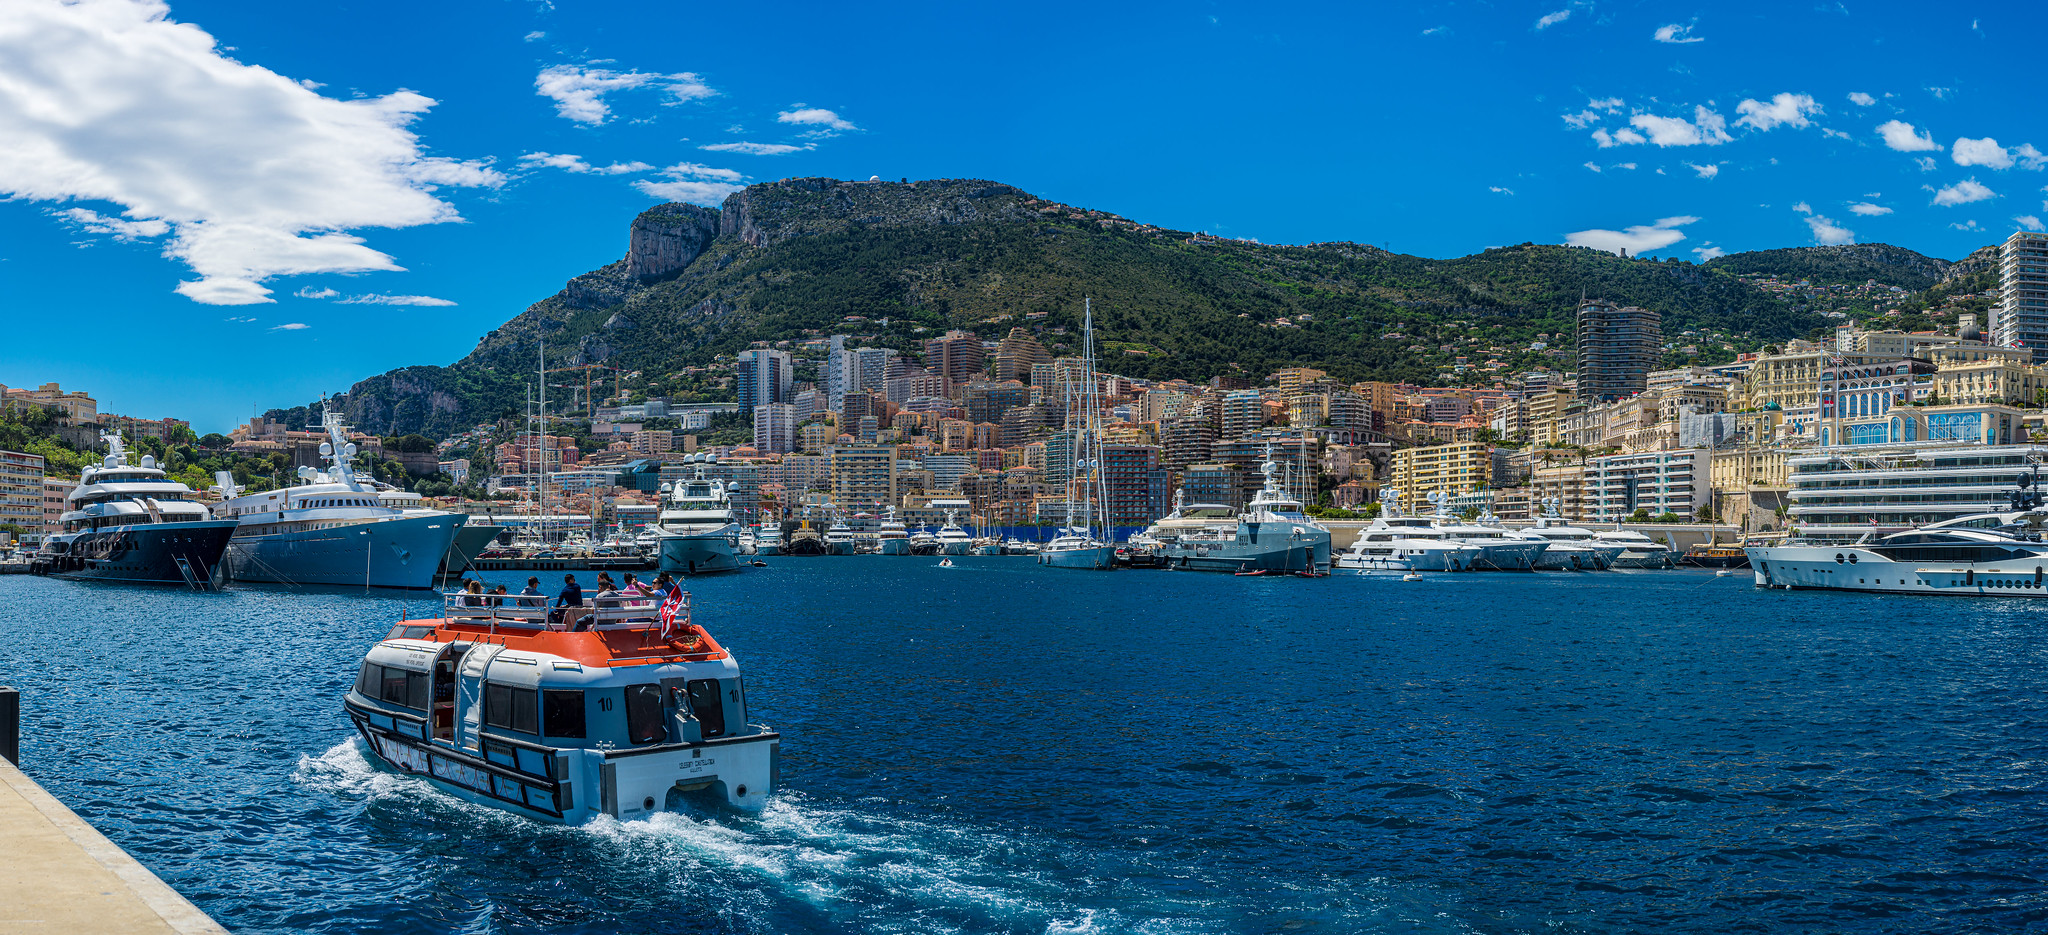
\includegraphics[width=8cm]{fig/lec04/Monte_Carlo_City.jpg}
\caption{Monte Carlo port \\(source: \href{https://www.flickr.com/photos/flynn_nrg/40890124713/}{www.flickr.com}, by \href{https://www.flickr.com/photos/flynn_nrg/}{Miguel Mendez} \href{https://creativecommons.org/licenses/by/2.0/}{CC BY 2.0})}
\label{fig:MMonte_Carlo_City}
\end{figure}
}

%%%%%%%%%%%%%%%%%%%%%%%%%%%%%%%%%%%%%%%%%%%%%%%%%%%%%%%%%%%%%%%%%%
\section{Basic Monte Carlo Prediction} 
%%%%%%%%%%%%%%%%%%%%%%%%%%%%%%%%%%%%%%%%%%%%%%%%%%%%%%%%%%%%%%%%%%
\begin{frame}
\frametitle{Table of Contents}
\tableofcontents[currentsection]
\end{frame}

%%%%%%%%%%%%%%%%%%%%%%%%%%%%%%%%%%%%%%%%%%%%%%%%%%%%%%%%%%%%%
%% Task Description and Basic Solution %%
%%%%%%%%%%%%%%%%%%%%%%%%%%%%%%%%%%%%%%%%%%%%%%%%%%%%%%%%%%%%%
\frame{\frametitle{Task Description and Basic Solution}
\begin{block}{MC prediction problem statement}
\begin{itemize}
	\item Estimate state value $v_{\pi}(x)$ for a given policy $\pi$.
	\item Available are samples $\left\langle x_{k,j}, u_{k,j}, r_{k+1,j}\right\rangle$ for episodes  $j=1,\ldots,J$.
\end{itemize}
\end{block}
\pause
\vspace{0.25cm}
MC solution approach:
\begin{itemize}
	\item Average returns after visiting state $x_k$ over episodes $j=1,\ldots$
	\begin{equation}
		v_{\pi}(x_k) \approx \hat{v}_{\pi}(x_k)=\frac{1}{J}\sum_{j=1}^J g_{k,j}=\frac{1}{J}\sum_{j=1}^J\sum_{i=0}^{T_j} \gamma^i r_{k+i+1,j}\, .
		\label{eq:MC_average_v_basic}
	\end{equation}
	\item Above, $T_j$ denotes the \hl{terminating time step} of each episode $j$.\pause
	\item \hl{First-visit MC}: Apply \eqref{eq:MC_average_v_basic} only to the first state visit per episode.\pause
	\item \hl{Every-visit MC}: Apply \eqref{eq:MC_average_v_basic} each time visiting a certain state per episode (if a state is visited more than one time per episode).
\end{itemize}
}

%%%%%%%%%%%%%%%%%%%%%%%%%%%%%%%%%%%%%%%%%%%%%%%%%%%%%%%%%%%%%
%% Algorithmic Implementation:MC-Based Prediction %%
%%%%%%%%%%%%%%%%%%%%%%%%%%%%%%%%%%%%%%%%%%%%%%%%%%%%%%%%%%%%%
\frame{\frametitle{Algorithmic Implementation: MC-Based Prediction}
\setlength{\algomargin}{0.5em}
\begin{algorithm}[H]
\SetKwInput{Input}{input} 
\SetKwInput{Output}{output}
\SetKwInput{Init}{init}
\SetKwInput{Param}{parameter}
\Input{a policy $\pi$ to be evaluated}
\Output{estimate of $\bm{v}_{\mathcal{X}}^{\pi}$ (i.e. value estimate for all states				 $x\in\mathcal{X}$)}
\Init{$\hat{v}(x)\, \forall \, x\in\mathcal{X}$ arbitrary except $v_0(x)=0$ if $x$ is terminal\newline 
$l(x)\leftarrow$ an empty list for every $x\in\mathcal{X}$}
 \For{$j=1,\ldots,J$ episodes}{
		Generate an episode following $\pi$: $x_{0}, u_{0}, r_{1},\ldots,x_{T_j}, u_{T_j}, r_{T_{j}+1}$ \;
		Set $g \leftarrow 0$\;
		\For{$k=T_j-1, T_j-2, T_j-3,\ldots, 0$ time steps}{
			$g \leftarrow \gamma g + r_{k+1}$\;
			\If{$x_{k}\notin \left\langle x_{0}, x_{1}, \ldots, x_{k-1}\right\rangle$}{
					Append $g$ to list $l(x_k)$\;
					$\hat{v}(x_k)\leftarrow \mbox{average}(\,l(x_k)\,)$\;}
		}
	}
\caption{First-visit MC state-value prediction}
\label{algo:MC_state_prediction_first_visit}
\end{algorithm}
}

%%%%%%%%%%%%%%%%%%%%%%%%%%%%%%%%%%%%%%%%%%%%%%%%%%%%%%%%%%%%%
%% Incremental Implementation%%
%%%%%%%%%%%%%%%%%%%%%%%%%%%%%%%%%%%%%%%%%%%%%%%%%%%%%%%%%%%%%
\frame{\frametitle{Incremental Implementation}
\begin{itemize}
	\item \algoref{algo:MC_state_prediction_first_visit} is inefficient due to large memory demand.
	\item Better: use \hl{incremental / recursive implementation}.\pause
	\item The sample mean $\mu_1,\mu_2,\ldots$ of an arbitrary sequence $g_1, g_2, \ldots$ is:
\end{itemize}
\begin{equation}
	\begin{split}
		\mu_j &= \frac{1}{j}\sum_{i=1}^j g_i,\\
					&= \frac{1}{j}\left[g_j + \sum_{i=1}^{j-1} g_i\right],\\
					&= \frac{1}{j}\left[g_j + (j-1) \mu_{j-1}\right],\\
					&=\mu_{j-1} + \frac{1}{j}\left[g_j-\mu_{j-1}\right].
	\end{split}
	\label{eq:inc_impl_MC_pred}
\end{equation} \pause
\begin{itemize}
	\item \hl{If a given decision problem is non-stationary}, using a forgetting factor $\alpha\in\left\{\mathbb{R}|0<\alpha<1\right\}$ allows for dynamic adaption: 
\end{itemize}
\begin{equation}
	\mu_j = \mu_{j-1} + \alpha\left[g_j-\mu_{j-1}\right] .
	\label{eq:inc_impl_MC_pred_non_stat}
\end{equation}
}

%%%%%%%%%%%%%%%%%%%%%%%%%%%%%%%%%%%%%%%%%%%%%%%%%%%%%%%%%%%%%
%% Statistical Properties of MC-Based Prediction (1)%%
%%%%%%%%%%%%%%%%%%%%%%%%%%%%%%%%%%%%%%%%%%%%%%%%%%%%%%%%%%%%%
\frame{\frametitle{Statistical Properties of MC-Based Prediction (1)}
\onslide<1->{First-time visit MC:
\begin{itemize}
	\item Each return sample $g_j$ is independent from the others since they were drawn from separate episodes.   
	\item One receives \hl{i.i.d. data} to estimate $\E{\hat{v}_{\pi}}$ and consequently this \hl{is bias-free}.
	\item The estimate's variance $\Var{\hat{v}_{\pi}}$ drops with $1/n$ ($n$: available samples). 
\end{itemize}}
\onslide<2->{Every-time visit MC:
\begin{itemize}
	\item Each return sample $g_j$ is not independent from the others since they might be obtained from same episodes.   
	\item One receives \hl{non-i.i.d.} data to estimate $\E{\hat{v}_{\pi}}$ and consequently this \hl{is biased} for any $n<\infty$.
	\item Only in the limit $n\rightarrow \infty$ one receives $\left(v_{\pi}(x)-\E{\hat{v}_{\pi}(x)}\right) \rightarrow 0$.
\end{itemize}}
\footnotesize
\vspace{0.5cm}
\onslide<1->More information: S. Singh and  R. Sutton, "Reinforcement Learning with Replacing Eligibility Traces", Machine Learning, Vol. 22, pp. 123-158, 1996  
}

%%%%%%%%%%%%%%%%%%%%%%%%%%%%%%%%%%%%%%%%%%%%%%%%%%%%%%%%%%%%%
%% Statistical Properties of MC-Based Prediction (2)%%
%%%%%%%%%%%%%%%%%%%%%%%%%%%%%%%%%%%%%%%%%%%%%%%%%%%%%%%%%%%%%
\frame{\frametitle{Statistical Properties of MC-Based Prediction (2)}

\begin{itemize}
	\item State-value estimates for each state are independent.
	\item One estimate does not rely on the estimate of other states \newline(\hl{no bootstrapping} compared to DP).
	\item Makes MC particularly attractive when one requires state-value knowledge of only one or few states.
	\begin{itemize}
		\item Hence, generating episodes starting from the state of interest.
	\end{itemize}
\end{itemize}
\begin{figure}
	\subfloat{
		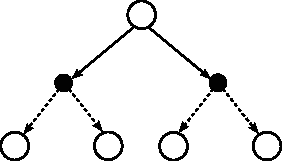
\includegraphics[height=2.5cm]{fig/lec04/Back_Up_DP.pdf}
	}
	\hspace{1cm}
	\subfloat{
		
\includegraphics[height=2.5cm]{fig/lec04/Back_Up_MC.pdf}
	}
\caption{Back-up diagrams for DP (left) and MC (right) prediction: shallow one-step back-ups with bootstrapping vs. deep back-ups over full epsiodes}
\end{figure}
}

%%%%%%%%%%%%%%%%%%%%%%%%%%%%%%%%%%%%%%%%%%%%%%%%%%%%%%%%%%%%%
%% MC-Based Predction Example: Forest Tree MDP%%
%%%%%%%%%%%%%%%%%%%%%%%%%%%%%%%%%%%%%%%%%%%%%%%%%%%%%%%%%%%%%
\frame{\frametitle{MC-Based Prediction Example: Forest Tree MDP (1)}
Let's reuse the forest tree MDP example with \textit{fifty-fifty policy} and discount factor $\gamma=0.8$
plus disaster probability $\alpha=0.2$:
\vspace{0.5cm}
\begin{figure}		
	%\hspace*{-1.5cm}
	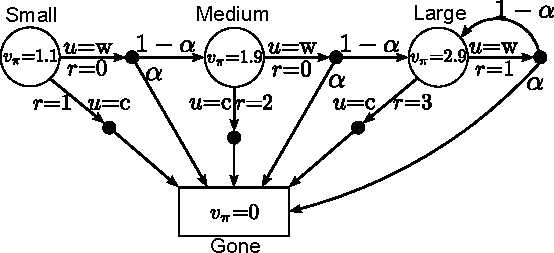
\includegraphics[width=9cm]{fig/lec04/Forest_Markov_Decision_Process_State_Value.pdf}
	\caption{Forest MDP with fifty-fifty-policy including state values}
\end{figure}
}

%%%%%%%%%%%%%%%%%%%%%%%%%%%%%%%%%%%%%%%%%%%%%%%%%%%%%%%%%%%%%
%% MC-Based Predction Example: Forest Tree MDP%%
%%%%%%%%%%%%%%%%%%%%%%%%%%%%%%%%%%%%%%%%%%%%%%%%%%%%%%%%%%%%%
\frame{\frametitle{MC-Based Prediction Example: Forest Tree MDP (2)}

\begin{figure}		
	%\hspace*{-1.5cm}
	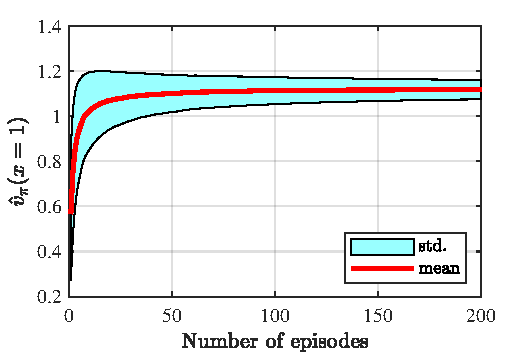
\includegraphics{fig/lec04/Forest_Tree_MC_Value_Prediction.pdf}
	\caption{State-value estimate of forest tree MDP initial state using MC-based prediction over the number of episodes being evaluated (mean and standard deviation are calculated based on 2000 independent runs)}
	\label{fig:Forest_Tree_MC_Value_Prediction}
\end{figure}
}

%%%%%%%%%%%%%%%%%%%%%%%%%%%%%%%%%%%%%%%%%%%%%%%%%%%%%%%%%%%%%
%% MC-Based Predction Example: Blackjack (1) %%
%%%%%%%%%%%%%%%%%%%%%%%%%%%%%%%%%%%%%%%%%%%%%%%%%%%%%%%%%%%%%
\frame{\frametitle{MC-Based Prediction Example: Blackjack (1)}
\begin{itemize}
	\item \hl{States} (200 in total)
	\begin{itemize}
		\item Player's sum: 12-21 (automatically twist if player's sum $<$ 12)
		\item Usable ace (counts 1/11): yes/no 
		\item Dealer's initial card: ace-10
	\end{itemize}\pause
	\item Action \hl{stick}: stop receiving cards (terminate episode)\pause
	\item Reward for \hl{stick}:
	\begin{itemize}
		\item +1 if player's sum $>$ dealer's sum
		\item 0 if player's sum $=$ dealer's sum
		\item -1 if player's sum $<$ dealer's sum
	\end{itemize}\pause
	\item Action \hl{twist/hit}: take another card (assuming no replacements)\pause
	\item Reward for \hl{twist/hit}:
	\begin{itemize}
		\item -1 if player's sum $>$  21 ('bust', terminates episode)
		\item 0 otherwise
	\end{itemize}\pause
	\item Dealer always sticks on any sum $\geq$ 17.
\end{itemize}
}

%%%%%%%%%%%%%%%%%%%%%%%%%%%%%%%%%%%%%%%%%%%%%%%%%%%%%%%%%%%%%
%% MC-Based Predction Example: Blackjack (2) %%
%%%%%%%%%%%%%%%%%%%%%%%%%%%%%%%%%%%%%%%%%%%%%%%%%%%%%%%%%%%%%
\frame{\frametitle{MC-Based Prediction Example: Blackjack (2)}
\begin{figure}
		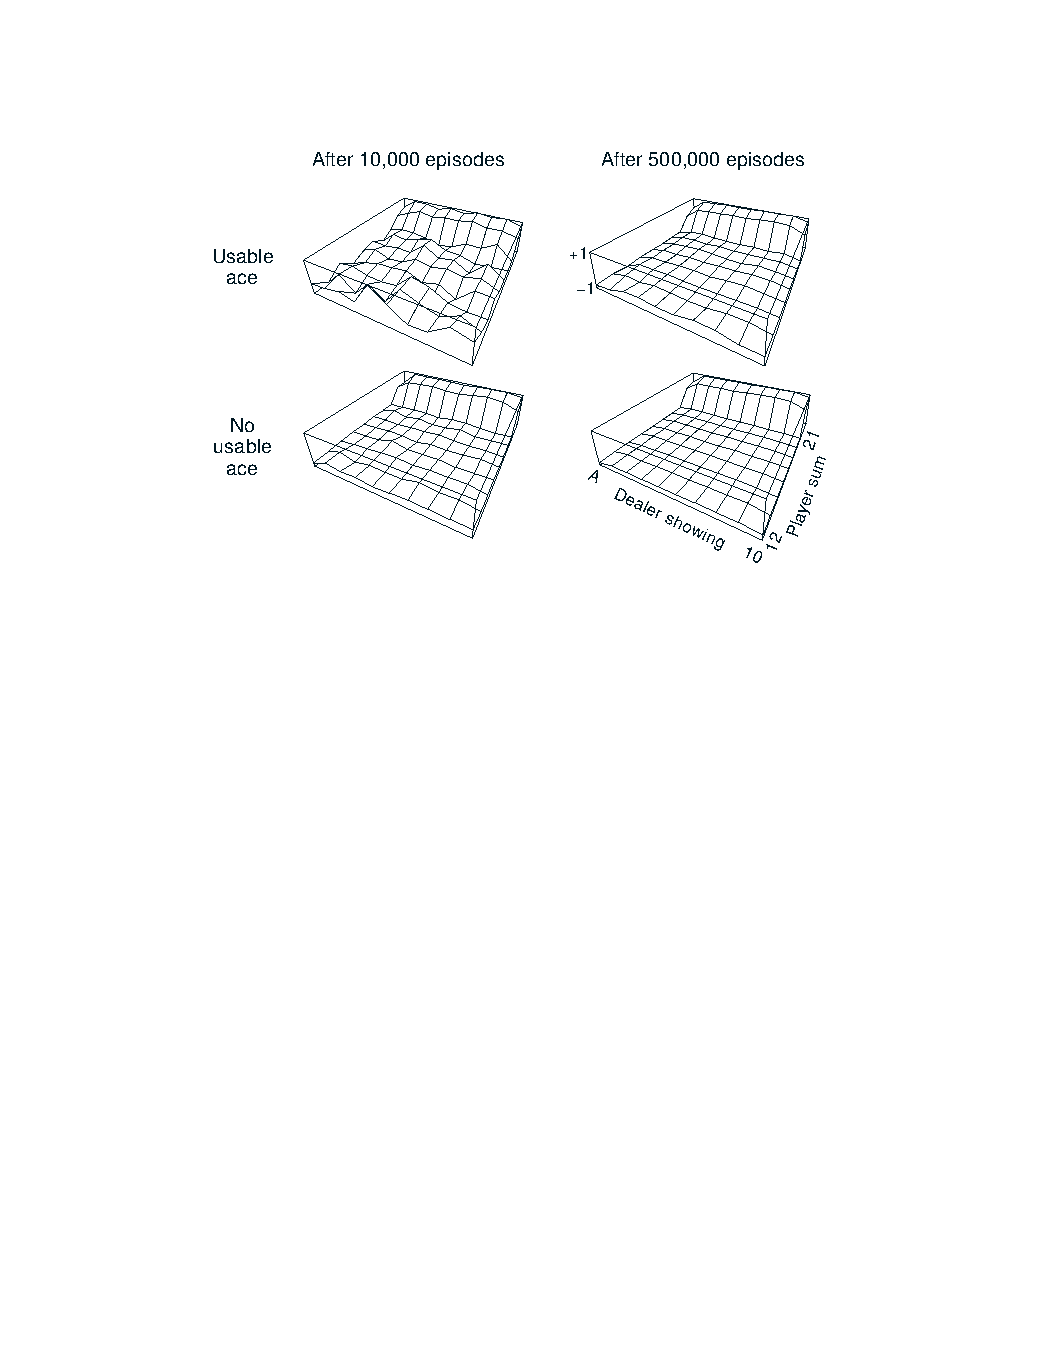
\includegraphics[width=9cm]{fig/lec04/MC_Black_Jack.pdf}
		\caption{Approximate state-value functions by first-visit MC prediction for a \hl{player's policy that sticks only on 20 or 21} (source: R. Sutton and G. Barto, Reinforcement learning: an introduction, 2018, \href{https://creativecommons.org/licenses/by-nc-nd/2.0/}{CC BY-NC-ND 2.0})}
		\label{fig:Blackjack_MC}
\end{figure}
}
%Remarks: 
%Blackjack could be modeled as a MDP since one has full knowledge of the system 'dynamics'
%Problem: Analytical/exact calculation of all transition probabilities not easy / a lot of work
%MC offers an alternative: set up a simulation environment with less effort in order bypass the need of calculating the transition probabilities

%%%%%%%%%%%%%%%%%%%%%%%%%%%%%%%%%%%%%%%%%%%%%%%%%%%%%%%%%%%%%
%% MC Estimation of Action Values %%
%%%%%%%%%%%%%%%%%%%%%%%%%%%%%%%%%%%%%%%%%%%%%%%%%%%%%%%%%%%%%
\frame{\frametitle{MC Estimation of Action Values}
Is a \hl{model available} (i.e. tuple $\left\langle\mathcal{X}, \mathcal{U}, \bm{\mathcal{P}}, \mathcal{R}, \gamma \right\rangle$)? 
\begin{itemize}
	\item \hl{Yes}: state values plus one-step prediction deliver optimal policy.
	\item \hl{No}: action values are very useful to directly obtain optimal choices.  
	\item Recap policy improvement from last lecture.
\end{itemize}\pause
\hl{Estimating $q{_\pi}(x, u)$} using MC approach:
\begin{itemize}
	\item Analog to state values summarized in \algoref{algo:MC_state_prediction_first_visit}.
	\item Only small extension: a visit refers to a state-action pair $(x, u)$.
	\item First-visit and every-visit variants exist.
\end{itemize}\pause
Possible problem when following a deterministic policy $\pi$:
\begin{itemize}
	\item Certain state-action pairs $(x, u)$ are never visited.
	\item Missing degree of exploration.\pause
	\item Workaround: \hl{exploring starts} i.e. starting episodes in random state-action pairs $(x, u)$ and thereafter following  $\pi$. 
\end{itemize}
}

%%%%%%%%%%%%%%%%%%%%%%%%%%%%%%%%%%%%%%%%%%%%%%%%%%%%%%%%%%%%%%%%%%
\section{Basic Monte Carlo Control} 
%%%%%%%%%%%%%%%%%%%%%%%%%%%%%%%%%%%%%%%%%%%%%%%%%%%%%%%%%%%%%%%%%%
\begin{frame}
\frametitle{Table of Contents}
\tableofcontents[currentsection]
\end{frame}

%%%%%%%%%%%%%%%%%%%%%%%%%%%%%%%%%%%%%%%%%%%%%%%%%%%%%%%%%%%%%
%% Applying Generalized Policy Iteration (GPI) to MC Control %%
%%%%%%%%%%%%%%%%%%%%%%%%%%%%%%%%%%%%%%%%%%%%%%%%%%%%%%%%%%%%%
\frame{\frametitle{Applying Generalized Policy Iteration (GPI) to MC Control}
\onslide<1->{GPI concept is directly applied to MC framework using action values:
\begin{equation}
\label{eq:GPI_MC}
	\pi_0 \rightarrow \hat{q}_{\pi_0} \rightarrow \pi_1 \rightarrow \hat{q}_{\pi_1} \rightarrow \cdots \pi^* \rightarrow \hat{q}_{\pi^*} \, .
\end{equation}}
\begin{itemize}
	\onslide<2->{\item Degree of freedom: Choose number of episodes to approximate $\hat{q}_{\pi_i}$.}
	\onslide<3->{\item Policy improvement is done by greedy choices:
	\begin{equation}
		\pi(x)= \argmax_{u} q(x, u) \quad \forall x\in\mathcal{X}\, .
	\end{equation}}
\end{itemize}
\onslide<1->{\begin{figure}
\begin{minipage}[c]{0.35\textwidth}
    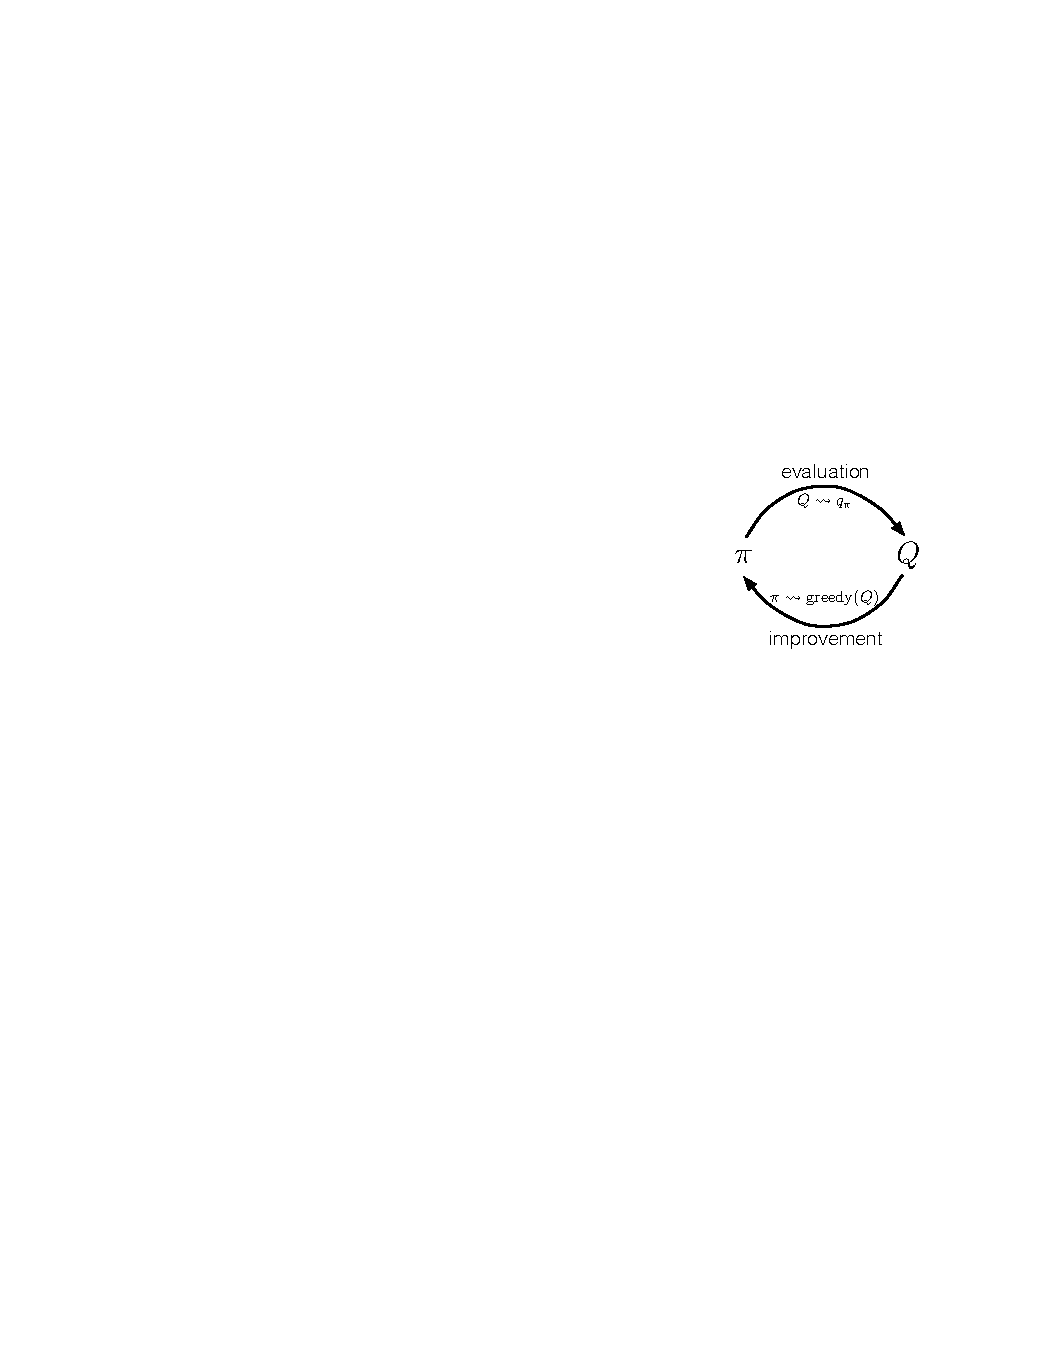
\includegraphics[width=4cm]{fig/lec04/MC_GPI.pdf}
  \end{minipage}\hfill
  \begin{minipage}[c]{0.65\textwidth}
    \caption{Transferring GPI to MC-based control (source: R. Sutton and G. Barto, Reinforcement learning: an introduction, 2018, \href{https://creativecommons.org/licenses/by-nc-nd/2.0/}{CC BY-NC-ND 2.0})}
		\label{fig:GPI_MC}
  \end{minipage}
\end{figure}}
}

%%%%%%%%%%%%%%%%%%%%%%%%%%%%%%%%%%%%%%%%%%%%%%%%%%%%%%%%%%%%%
%% Policy Improvement Theoreom %%
%%%%%%%%%%%%%%%%%%%%%%%%%%%%%%%%%%%%%%%%%%%%%%%%%%%%%%%%%%%%%
\frame{\frametitle{Policy Improvement Theorem}
Assuming that one is operating in an \hl{unknown MDP}, the policy improvement theorem \theoref{theo:Policy_improvement} is still valid for MC-based control:
\begin{block}{Policy improvement for MC-based control}
\begin{equation}
	\begin{split}
		q_{\pi_i}(x,\pi_{i+1}(x)) &= q_{\pi_i}(x,\argmax_{u} q_{\pi_i}(x,u)),\\
											&= \max_{u} q_{\pi_i}(x,u),\\
											&\geq q_{\pi_i}(x,\pi_{i}(x)),\\
											&\geq v_{\pi_i}(x).
	\end{split}
\end{equation} 
\end{block}
\begin{itemize}
	\item Each $\pi_{i+1}$ is uniformly better or just as good (if optimal) as $\pi_{i}$.
	\item Assumption: All state-action pairs are evaluated due to sufficient exploration.
	\begin{itemize}
		\item For example using exploring starts. 
	\end{itemize}
\end{itemize}
}

%%%%%%%%%%%%%%%%%%%%%%%%%%%%%%%%%%%%%%%%%%%%%%%%%%%%%%%%%%%%%
%% Algorithmic Implementation: MC-Based Control Using Exploring Start %%
%%%%%%%%%%%%%%%%%%%%%%%%%%%%%%%%%%%%%%%%%%%%%%%%%%%%%%%%%%%%%
\frame{\frametitle{Algorithmic Implementation: MC-Based Control}
\setlength{\algomargin}{0.5em}
\begin{algorithm}[H]
\footnotesize
\SetKwInput{Input}{input} 
\SetKwInput{Output}{output}
\SetKwInput{Init}{init}
\SetKwInput{Param}{parameter}
\Output{Optimal deterministic policy $\pi^*$}
\Init{$\pi_{i=0}(x)\in\mathcal{U}$ arbitrarily $\forall x\in\mathcal{X}$\newline
$\hat{q}(x,u)$ arbitrarily $\forall \, \left\{x\in\mathcal{X}, u\in\mathcal{U}\right\}$\newline 
$n(x,u)\leftarrow$ an empty list for state-action visits $\forall \, \left\{x\in\mathcal{X}, u\in\mathcal{U}\right\}$}
\Repeat{$\pi_{i+1} = \pi_{i}$}{
	$i\leftarrow i+1$ \;
	Choose $\left\{x_{0}, u_{0}\right\}$ randomly such that all pairs have probability $>$ 0 \;
	Generate an episode from $\left\{x_{0}, u_{0}\right\}$ following $\pi_{i}$ until termination step $T_i$\;
	Set $g \leftarrow 0$\;
	\For{$k=T_i-1, T_i-2, T_i-3,\ldots, 0$ time steps}{
				$g \leftarrow \gamma g + r_{k+1}$\;
				\If{$\left\{x_{k}, u_{k}\right\}\notin \left\langle \left\{x_{0}, u_{0}\right\}, \ldots, \left\{x_{k-1}, u_{k-1}\right\}\right\rangle$}{
						$n(x_k,u_k)\leftarrow n(x_k,u_k)+1$\;
						$\hat{q}(x_k,u_k)\leftarrow \hat{q}(x_k,u_k) + 1/n(x_k,u_k)\cdot(g-\hat{q}(x_k,u_k))$\;
						$\pi_{i}(x_k)\leftarrow\argmax_{u}\,\, \hat{q}(x_k,u)$\;
				}
	}
}
\caption{MC-based control using exploring starts (first-visit)}
\label{algo:MC_ES}
\end{algorithm}
}

%%%%%%%%%%%%%%%%%%%%%%%%%%%%%%%%%%%%%%%%%%%%%%%%%%%%%%%%%%%%%
%% MC-Based Control Example: Blackjack %%
%%%%%%%%%%%%%%%%%%%%%%%%%%%%%%%%%%%%%%%%%%%%%%%%%%%%%%%%%%%%%
\frame{\frametitle{MC-Based Control Example: Blackjack}
\begin{figure}
		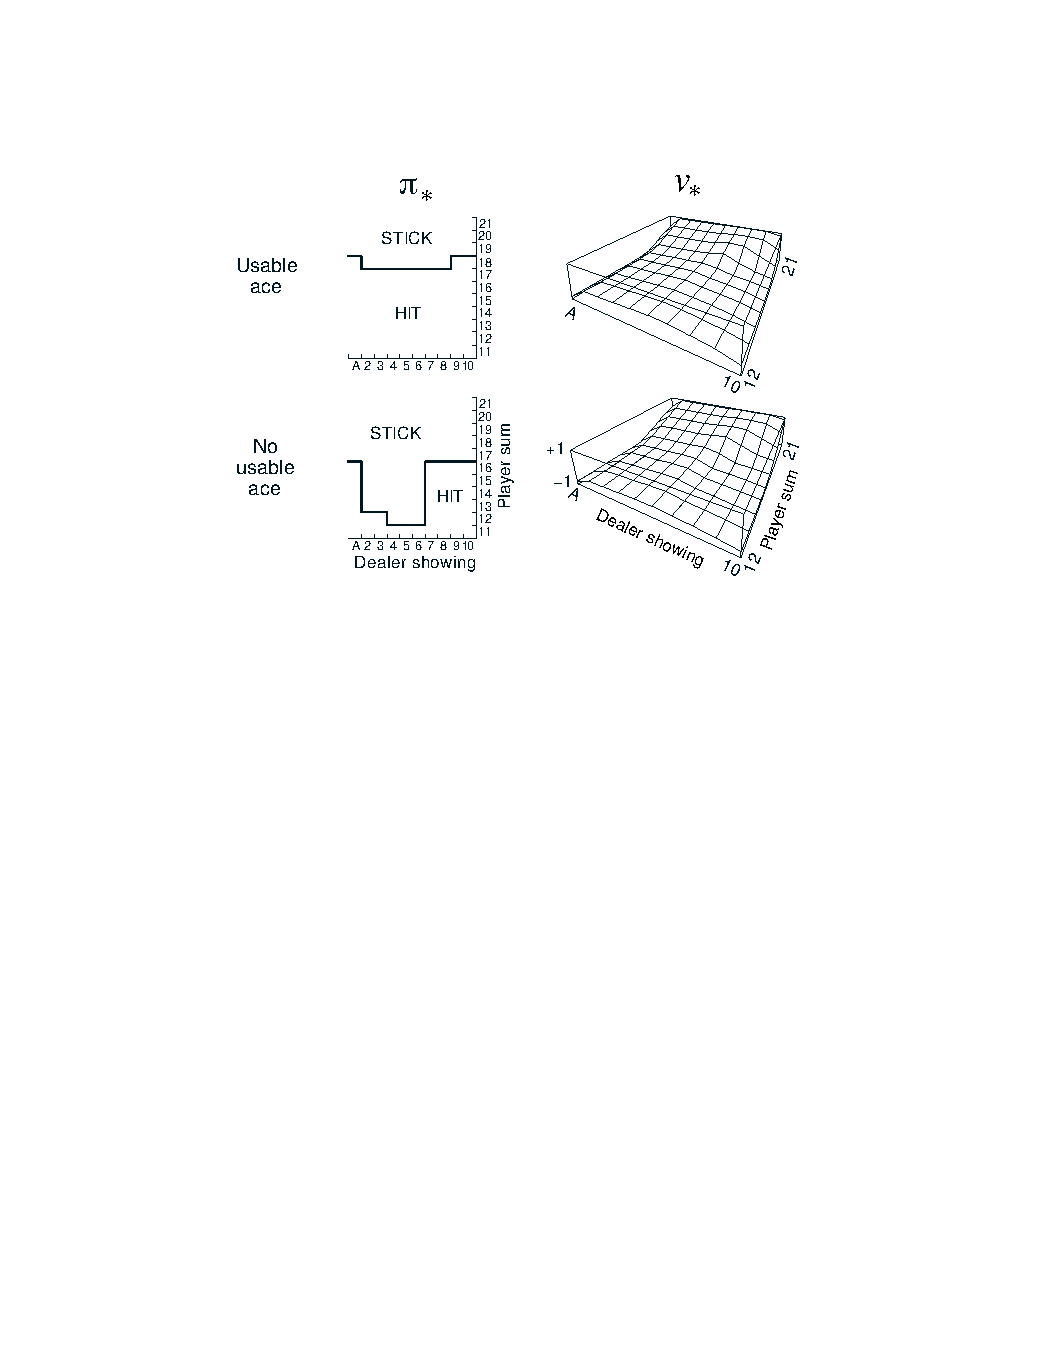
\includegraphics[width=9cm]{fig/lec04/MC_ES_Black_Jack.pdf}
		\caption{The optimal policy and state-value function for blackjack found by MC-based control using exploring starts. (source: R. Sutton and G. Barto, Reinforcement learning: an introduction, 2018, \href{https://creativecommons.org/licenses/by-nc-nd/2.0/}{CC BY-NC-ND 2.0})}
		\label{fig:MC_ES_Black_Jack}
\end{figure}
}

%%%%%%%%%%%%%%%%%%%%%%%%%%%%%%%%%%%%%%%%%%%%%%%%%%%%%%%%%%%%%%%%%%
\section{Extensions to Monte Carlo On-Policy Control} 
%%%%%%%%%%%%%%%%%%%%%%%%%%%%%%%%%%%%%%%%%%%%%%%%%%%%%%%%%%%%%%%%%%
\begin{frame}
\frametitle{Table of Contents}
\tableofcontents[currentsection]
\end{frame}

%%%%%%%%%%%%%%%%%%%%%%%%%%%%%%%%%%%%%%%%%%%%%%%%%%%%%%%%%%%%%
%% Off- and On-Policy Learning %%
%%%%%%%%%%%%%%%%%%%%%%%%%%%%%%%%%%%%%%%%%%%%%%%%%%%%%%%%%%%%%
\frame{\frametitle{Off- and On-Policy Learning}
\begin{itemize}
	\item \hl{On-policy learning}
	\begin{itemize}
		\item Evaluate or improve the policy used to make decisions.
		\item Agent picks own actions.
		\item Exploring starts (ES) is an on-policy method example.
		\item However: ES is a restrictive assumption and not always applicable \newline (in some cases the starting state-action pair cannot be choosen freely).
	\end{itemize}\pause
	\vspace{1cm}
	\item \hl{Off-policy learning}
		\begin{itemize}
		\item Evaluate or improve a policy different from that used to generate data.
		\item Agent cannot apply own actions.
		\item Will be focused in the next sections.
	\end{itemize}
\end{itemize}
}

%%%%%%%%%%%%%%%%%%%%%%%%%%%%%%%%%%%%%%%%%%%%%%%%%%%%%%%%%%%%%
%% Epsilon-Greedy as an On-Policy Alternative %%
%%%%%%%%%%%%%%%%%%%%%%%%%%%%%%%%%%%%%%%%%%%%%%%%%%%%%%%%%%%%%
\frame{\frametitle{$\varepsilon$-Greedy as an On-Policy Alternative}
\begin{itemize}
	\item Exploration requirement:
	\begin{itemize}
		\item Visit all state-action pairs with probability:
		\begin{equation}
			 \pi(u|x) > 0 \quad \forall\, \left\{x\in\mathcal{X}, u\in\mathcal{U}\right\}\, .
		\end{equation}
		\item Policies with this characteristic are called: \hl{soft}.
		\item Level of exploration can be tuned during the learning process.
	\end{itemize}\pause
	\vspace{0.5cm}
	\item \hl{$\varepsilon$-greedy on-policy learning} 
		\begin{itemize}
		\item With probability $\varepsilon$ the agent's choice (i.e. the policy output) is overwritten with a random action.
		\item Probability of all non-greedy actions: \begin{equation}\varepsilon/|\mathcal{U}|\,.\end{equation}
		\item Probability of the greedy action: \begin{equation}1-\varepsilon+\varepsilon/|\mathcal{U}|\,.\end{equation}
		\item Above, $|\mathcal{U}|$ is the cardinality of the action space.
	\end{itemize}
\end{itemize}
}

%%%%%%%%%%%%%%%%%%%%%%%%%%%%%%%%%%%%%%%%%%%%%%%%%%%%%%%%%%%%%
%% Algorithmic implementation $\varepsilon$-Greedy MC-Control %%
%%%%%%%%%%%%%%%%%%%%%%%%%%%%%%%%%%%%%%%%%%%%%%%%%%%%%%%%%%%%%
\frame{\frametitle{Algorithmic Implementation $\varepsilon$-Greedy MC-Control}
\vspace{-0.2cm}
\setlength{\algomargin}{0.5em}
\begin{algorithm}[H]
\footnotesize
\SetKwInput{Input}{input} 
\SetKwInput{Output}{output}
\SetKwInput{Init}{init}
\SetKwInput{Param}{parameter}
\Output{Optimal $\varepsilon$-greedy policy $\pi^*(u|x)$}
\Param{$\varepsilon\in\left\{\mathbb{R}|0<\varepsilon<<1\right\}$}
\Init{$\pi_{i=0}(u|x)$ arbitrarily soft $\forall \, \left\{x\in\mathcal{X}, u\in\mathcal{U}\right\}$\newline
$\hat{q}(x,u)$ arbitrarily $\forall \, \left\{x\in\mathcal{X}, u\in\mathcal{U}\right\}$\newline 
$n(x,u)\leftarrow$ an empty list counting state-action visits $\forall \, \left\{x\in\mathcal{X}, u\in\mathcal{U}\right\}$}
\Repeat{$\pi_{i+1} = \pi_{i}$}{
	Generate an episode following $\pi_i$: $x_{0}, u_{0}, r_{1},\ldots,x_{T_j}, u_{T_j}, r_{T_{j+1}}$ \;
	$i\leftarrow i+1$ \;
	Set $g \leftarrow 0$\;
	\For{$k=T_i-1, T_i-2, T_i-3,\ldots, 0$ time steps}{
				$g \leftarrow \gamma g + r_{k+1}$\;
				\If{$\left\{x_{k}, u_{k}\right\}\notin \left\langle \left\{x_{0}, u_{0}\right\}, \ldots, \left\{x_{k-1}, u_{k-1}\right\}\right\rangle$}{
						$n(x_k,u_k)\leftarrow n(x_k,u_k)+1$\;
						$\hat{q}(x_k,u_k)\leftarrow \hat{q}(x_k,u_k) + 1/n(x_k,u_k)\cdot(g-\hat{q}(x_k,u_k))$\;
						$\tilde{u}\leftarrow\argmax_{u}\,\, \hat{q}(x_k,u)$\;
						$\pi_i(u|x_k)\leftarrow\begin{cases}1-\varepsilon+\varepsilon/|\mathcal{U}|, \quad u=\tilde{u}\\ \varepsilon/|\mathcal{U}|, \quad u\neq\tilde{u}\end{cases}$\;
				}
	}
}
\caption{MC-based control using $\varepsilon$-greedy approach}
\label{algo:MC_eps_greedy}
\end{algorithm}
}

%%%%%%%%%%%%%%%%%%%%%%%%%%%%%%%%%%%%%%%%%%%%%%%%%%%%%%%%%%%%%
%% $\varepsilon$-Greedy Policy Improvement (1)%%
%%%%%%%%%%%%%%%%%%%%%%%%%%%%%%%%%%%%%%%%%%%%%%%%%%%%%%%%%%%%%
\frame{\frametitle{$\varepsilon$-Greedy Policy Improvement (1)}
\begin{theo}{Policy improvement for $\varepsilon$-greedy policy}{policy_improv_eps_greedy}
Given an MDP, for any $\varepsilon$-greedy policy $\pi$ the $\varepsilon$-greedy policy $\pi'$ with respect to $q_\pi$ is an improvement, i.e. $v_{\pi'} > v_{\pi} \quad \forall x\in\mathcal{X}$.
\end{theo}\pause
Small proof:
\small
\begin{equation}
	\begin{split}
		q_{\pi}(x,\pi'(x)) &= \sum_{u}\pi'(u|x)q_{\pi}(x,u),\\
											&= \frac{\varepsilon}{|\mathcal{U}|}\sum_{u}q_{\pi}(x,u) + (1-\varepsilon)\max_{u}q_{\pi}(x,u),\\
											&\geq \frac{\varepsilon}{|\mathcal{U}|}\sum_{u}q_{\pi}(x,u) + (1-\varepsilon)\sum_{u}\frac{\pi(u|x)-\frac{\varepsilon}{|\mathcal{U}|}}{1-\varepsilon}q_{\pi}(x,u).
\end{split}
\end{equation} 
\normalsize
In the inequality line, the second term is the weighted sum over action values given an $\varepsilon$-greedy policy. This weighted sum will be always smaller or equal than  $\max_{u}q_{\pi}(x,u)$.
}

%%%%%%%%%%%%%%%%%%%%%%%%%%%%%%%%%%%%%%%%%%%%%%%%%%%%%%%%%%%%%
%% $\varepsilon$-Greedy Policy Improvement (2)%%
%%%%%%%%%%%%%%%%%%%%%%%%%%%%%%%%%%%%%%%%%%%%%%%%%%%%%%%%%%%%%
\frame{\frametitle{$\varepsilon$-Greedy Policy Improvement (2)}
Continuation:
\small
\begin{equation}
	\begin{split}
		q_{\pi}(x,\pi'(x)) &\geq \frac{\varepsilon}{|\mathcal{U}|}\sum_{u}q_{\pi}(x,u) + (1-\varepsilon)\sum_{u}\frac{\pi(u|x)-\frac{\varepsilon}{|\mathcal{U}|}}{1-\varepsilon}q_{\pi}(x,u),\\
											&= \frac{\varepsilon}{|\mathcal{U}|}\sum_{u}\left(q_{\pi}(x,u) - q_{\pi}(x,u)\right) + \sum_{u}\pi(u|x)q_{\pi}(x,u),\\
											&=\sum_{u}\pi(u|x)q_{\pi}(x,u),\\
											&=v_{\pi}(x).
	\end{split}
\end{equation} 
\normalsize\pause
\begin{itemize}
	\item Policy improvement theorem is still valid when comparing $\varepsilon$-greedy policies against each other.
	\item But: There might be a non-$\varepsilon$-greedy policy which is better. 
\end{itemize}
}

%%%%%%%%%%%%%%%%%%%%%%%%%%%%%%%%%%%%%%%%%%%%%%%%%%%%%%%%%%%%%
%% MC-Based Control Example: Forest Tree MDP (1)%%
%%%%%%%%%%%%%%%%%%%%%%%%%%%%%%%%%%%%%%%%%%%%%%%%%%%%%%%%%%%%%
\frame{\frametitle{MC-Based Control Example: Forest Tree MDP (1)}
\vspace{-0.5cm}
\begin{figure}		
	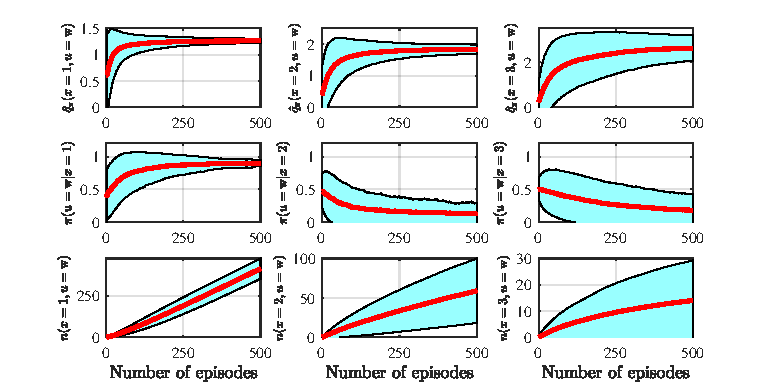
\includegraphics{fig/lec04/Forest_Tree_MC_Control_eps_02.pdf}
	\caption{Different estimates of forest tree MDP ($\alpha=0.2, \gamma=0.8$) using MC control with \hl{$\varepsilon=0.2$} over the number of episodes. Mean is red and standard deviation is light blue, both calculated based on 2000 independent uns.}
	\label{fig:Forest_Tree_MC_Control_eps_02}
\end{figure}
}

%%%%%%%%%%%%%%%%%%%%%%%%%%%%%%%%%%%%%%%%%%%%%%%%%%%%%%%%%%%%%
%% MC-Based Control Example: Forest Tree MDP (2)%%
%%%%%%%%%%%%%%%%%%%%%%%%%%%%%%%%%%%%%%%%%%%%%%%%%%%%%%%%%%%%%
\frame{\frametitle{MC-Based Control Example: Forest Tree MDP (2)}
\vspace{-0.5cm}
\begin{figure}		
	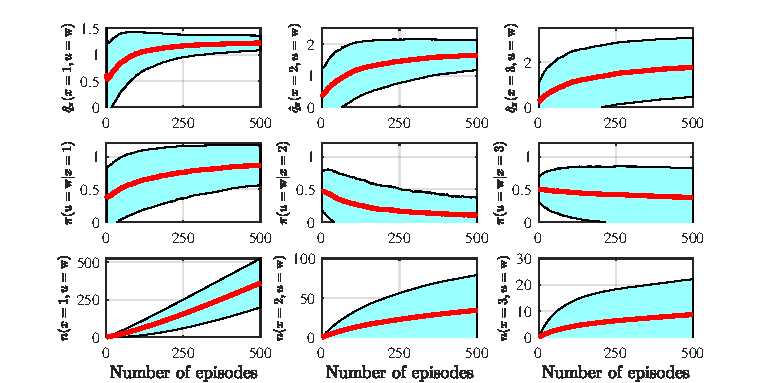
\includegraphics{fig/lec04/Forest_Tree_MC_Control_eps_005.pdf}
	\caption{Different estimates of forest tree MDP ($\alpha=0.2, \gamma=0.8$) using MC control with \hl{$\varepsilon=0.05$} over the number of episodes. Mean is red and standard deviation is light blue, both calculated based on 2000 independent runs.}
	\label{fig:Forest_Tree_MC_Control_eps_005}
\end{figure}
}

%%%%%%%%%%%%%%%%%%%%%%%%%%%%%%%%%%%%%%%%%%%%%%%%%%%%%%%%%%%%%
%% MC-Based Control Example: Forest Tree MDP (3)%%
%%%%%%%%%%%%%%%%%%%%%%%%%%%%%%%%%%%%%%%%%%%%%%%%%%%%%%%%%%%%%
\frame{\frametitle{MC-Based Control Example: Forest Tree MDP (3)}
Observations on forest tree MDP with $\varepsilon$-greedy MC-based control:
\begin{itemize}
	\item Rather slow convergence rate: quite a number of episodes is required. \pause
	\item Significant uncertainty present in a single sequence. \pause
	\item Later states are less often visited and, therefore, more uncertain. \pause
	\item Exploration is controlled by $\varepsilon$: in a totally greedy policy the state $x=3$ is not visited at all (cf. \figref{fig:Forest_Markov_Decision_Process_Optimal_Action_Value}). With $\varepsilon$-greedy this state is visited occasionally. \pause
	\item Nevertheless, the above figures highlight that MC-based control for the forest tree MDP tend towards the optimal policies discovered by dynamic programming (cf. \tabref{tab:Forest_tree_value_iteration}). 
\end{itemize}
}

%%%%%%%%%%%%%%%%%%%%%%%%%%%%%%%%%%%%%%%%%%%%%%%%%%%%%%%%%%%%%
%% Greedy in the Limit with Infinite Exploration (GLIE) %%
%%%%%%%%%%%%%%%%%%%%%%%%%%%%%%%%%%%%%%%%%%%%%%%%%%%%%%%%%%%%%
\frame{\frametitle{Greedy in the Limit with Infinite Exploration (GLIE)}
\begin{defi}{Greedy in the limit with infinite exploration (GLIE)}{GLIE}
A learning policy $\pi$ is called GLIE if it satisfies the following two properties:
\begin{itemize}
	\item If a state is visited infinitely often, then each action is chosen infinitely often:
	\begin{equation}
		\lim_{i\rightarrow\infty} \pi_i(u|x)=1 \quad \forall \, \left\{x\in\mathcal{X}, u\in\mathcal{U}\right\}\, .
	\end{equation}
	\item In the limit ($i\rightarrow \infty$) the learning policy is greedy with respect to the learned action value:
	\begin{equation}
		\lim_{i\rightarrow\infty} \pi_i(u|x)=\pi(x)= \argmax_{u} q(x, u) \quad \forall x\in\mathcal{X} \, .
	\end{equation}
\end{itemize}
\end{defi}
}

%%%%%%%%%%%%%%%%%%%%%%%%%%%%%%%%%%%%%%%%%%%%%%%%%%%%%%%%%%%%%
%% GlIE Monte-Carlo Control %%
%%%%%%%%%%%%%%%%%%%%%%%%%%%%%%%%%%%%%%%%%%%%%%%%%%%%%%%%%%%%%
\frame{\frametitle{GLIE Monte Carlo Control}
\begin{theo}{Optimal decision using MC-control with $\varepsilon$-greedy}{GLIE_MC}
MC-based control using $\varepsilon$-greedy exploration is GLIE, if $\varepsilon$ is decreased at rate
\begin{equation}
	\varepsilon_i = \frac{1}{i}
\end{equation}
with $i$ being the increasing episode index. In this case,
\begin{equation}
	\hat{q}(x, u) = q^*(x, u)
\end{equation}
follows.
\end{theo}
\pause
Remarks:
\begin{itemize}
	\item Limited feasibility: infinite number of episodes required.
	\item $\varepsilon$-greedy is an undirected exploration strategy. Can that be the most efficient way of learning?
\end{itemize}
}

%%%%%%%%%%%%%%%%%%%%%%%%%%%%%%%%%%%%%%%%%%%%%%%%%%%%%%%%%%%%%%%%%%
\section{Monte Carlo Off-Policy Prediction} 
%%%%%%%%%%%%%%%%%%%%%%%%%%%%%%%%%%%%%%%%%%%%%%%%%%%%%%%%%%%%%%%%%%
\begin{frame}
\frametitle{Table of Contents}
\tableofcontents[currentsection]
\end{frame}

%%%%%%%%%%%%%%%%%%%%%%%%%%%%%%%%%%%%%%%%%%%%%%%%%%%%%%%%%%%%%
%% Off-Policy Learning Background %%
%%%%%%%%%%%%%%%%%%%%%%%%%%%%%%%%%%%%%%%%%%%%%%%%%%%%%%%%%%%%%
\frame{\frametitle{Off-Policy Learning Background}
Drawback of on-policy learning:
\begin{itemize}
	\item Only a compromise: comes with inherent exploration but at the cost of learning action values for a \hl{near-optimal policy}. 
\end{itemize}
\vspace{0.75cm}\pause
Idea off-policy learning:
\begin{itemize}
	\item Use two separated policies:
	\begin{itemize}
		\item \hl{Behavior policy} $b(u|x)$: Explores in order to generate experience.
		\item \hl{Target policy} $\pi(u|x)$: Learns from that experience to become the optimal policy.
	\end{itemize}\pause
	\item Use cases:
	\begin{itemize}
		\item Learn from observing humans or other agents/controllers.
		\item Re-use experience generated from old policies ($\pi_0,\pi_1,\ldots$).
		\item Learn about multiple policies while following one policy.
	\end{itemize}
\end{itemize}
}

%%%%%%%%%%%%%%%%%%%%%%%%%%%%%%%%%%%%%%%%%%%%%%%%%%%%%%%%%%%%%
%% Off-Policy Prediction Problem Statement %%
%%%%%%%%%%%%%%%%%%%%%%%%%%%%%%%%%%%%%%%%%%%%%%%%%%%%%%%%%%%%%
\frame{\frametitle{Off-Policy Prediction Problem Statement}
\begin{block}{MC off-policy prediction problem statement}
\begin{itemize}
	\item Estimate $v_\pi$ and/or $q_\pi$ while following $b(u|x)$.
	\item Both policies are considered fixed (prediction assumption).
\end{itemize}
\end{block}
\vspace{0.75cm}\pause
Requirement:
\begin{itemize}
	\item \hl{Coverage}: Every action taken under $\pi$ must be (at least occasionally) taken under $b$, too. Hence, it follows:
	\begin{equation}
		\pi(u|x) > 0 \Rightarrow b(u|x) > 0 \quad \forall \, \left\{x\in\mathcal{X}, u\in\mathcal{U}\right\} .
	\end{equation}\pause
	\item Consequences from that:
	\begin{itemize}
		\item In any state $b$ is not identical to $\pi$, $b$ must be stochastic.
		\item Nevertheless: $\pi$ might be deterministic (e.g. control applications) or stochastic.
	\end{itemize}
\end{itemize}
}

%%%%%%%%%%%%%%%%%%%%%%%%%%%%%%%%%%%%%%%%%%%%%%%%%%%%%%%%%%%%%
%% Importance Sampling %%
%%%%%%%%%%%%%%%%%%%%%%%%%%%%%%%%%%%%%%%%%%%%%%%%%%%%%%%%%%%%%
\frame{\frametitle{Importance Sampling}
What is the probability of observing a certain trajectory on random variables $U_k, X_{k+1}, U_{k+1}, \ldots, X_{T}$ starting in $X_{k}$ while following $\pi$?
\begin{equation}
\begin{split}
	&\Pb{U_k, X_{k+1}, U_{k+1}, \ldots , X_{T}| X_{k}, \pi},\\
	=&\pi(U_k|X_{k})p(X_{k+1}|X_{k}, U_{k})\pi(U_{k+1}|X_{k+1})\cdots\,,\\
	=&\prod_k^{T-1} \pi(U_k|X_{k})p(X_{k+1}|X_{k}, U_{k}).
	\end{split}
\end{equation}
Above $p$ is the state-transition probability (cf. \defref{defi:Markov_decision_process}).\pause
\begin{defi}{Importance sampling ratio}{import_sampl_ratio}
The relative probability of a trajectory under the target and behavior policy, the importance sampling ratio, from sample step $k$ to $T$ is:
\begin{equation}
	\rho_{k:T}=\frac{\prod_k^{T-1} \pi(U_k|X_{k})p(X_{k+1}|X_{k}, U_{k})}{\prod_k^{T-1} b(U_k|X_{k})p(X_{k+1}|X_{k}, U_{k})}=\frac{\prod_k^{T-1} \pi(U_k|X_{k})}{\prod_k^{T-1} b(U_k|X_{k})} .
	\label{eq:import_sampl_ratio}
\end{equation}
\end{defi}
}

%%%%%%%%%%%%%%%%%%%%%%%%%%%%%%%%%%%%%%%%%%%%%%%%%%%%%%%%%%%%%
%% Importance Sampling for Monte Carlo Prediction (1)%%
%%%%%%%%%%%%%%%%%%%%%%%%%%%%%%%%%%%%%%%%%%%%%%%%%%%%%%%%%%%%%
\frame{\frametitle{Importance Sampling for Monte Carlo Prediction (1)}
\begin{defi}{State-value estimation via Monte Carlo importance sampling}{MC_ord_import_sampl}
Estimating the state value $v_\pi$ following a behavior policy $b$ using (ordinary) importance sampling (OIS) results in scaling and averaging the sampled returns by the importance sampling ratio per episode:
\begin{equation}
	\hat{v}_\pi(x_k)=\frac{\sum_{k\in\mathcal{T}(x_k)}\rho_{k:T(k)}g_k}{|\mathcal{T}(x_k)|}.
	\label{eq:OIS}
\end{equation}
\end{defi}
Notation remark:
\begin{itemize}
	\item $\mathcal{T}(x_k)$: set of all time steps in which the state $x_k$ is visited the first or each time per episode.
	\item $T(k)$: Termination of a specific episode starting from $k$.
\end{itemize}\pause
General remark:
\begin{itemize}
	\item From \eqref{eq:import_sampl_ratio} it can be seen that $\hat{v}$ is bias-free (first-visit assumption).
	\item However, if $\rho$ is large (distinctly different policies) the estimate's variance is large (i.e. uncertain for small numbers of samples).
\end{itemize}
}

%%%%%%%%%%%%%%%%%%%%%%%%%%%%%%%%%%%%%%%%%%%%%%%%%%%%%%%%%%%%%
%% Importance Sampling for Monte Carlo Prediction (2)%%
%%%%%%%%%%%%%%%%%%%%%%%%%%%%%%%%%%%%%%%%%%%%%%%%%%%%%%%%%%%%%
\frame{\frametitle{Importance Sampling for Monte Carlo Prediction (2)}
\begin{defi}{Weighted importance sampling for MC-based prediction}{MC_weighted_import_sampl}
Estimating the state value $v_\pi$ following a behavior policy $b$ using weighted importance sampling (WIS) results in a scaling and a weighted averaging of the sampled returns by the importance sampling ratio per episode:
\begin{equation}
\begin{split}
	\hat{v}_\pi(x_k)= \begin{cases}\frac{\sum_{k\in\mathcal{T}(x_k)}\rho_{k:T(k)}g_k}{\sum_{k\in\mathcal{T}(x_k)}\rho_{k:T(k)}}, \quad &\mbox{if}\,\,\sum_{k\in\mathcal{T}(x_k)}\rho_{k:T(k)}\neq0 \\ 0, &\mbox{if}\,\,\sum_{k\in\mathcal{T}(x_k)}\rho_{k:T(k)} = 0\quad \end{cases}.
\end{split}
\label{eq:WIS_MC}
\end{equation}
\end{defi}\pause
Comparison to OIS:
\begin{itemize}
	\item Weighting introduces bias (which reduces to zero in the limit).\pause
	\item But: weighting limits variance while the OIS's variance is unbounded.
	\begin{itemize}
		\item Largest weight per return sample for WIS is one, while OIS's weights are unbounded. 
	\end{itemize}\pause
	\item Conclusion: WIS delivers 'better' estimates for few samples and, therefore, is often preferred in practice.
\end{itemize}
}

%%%%%%%%%%%%%%%%%%%%%%%%%%%%%%%%%%%%%%%%%%%%%%%%%%%%%%%%%%%%%
%% Importance Sampling Example: Blackjack%%
%%%%%%%%%%%%%%%%%%%%%%%%%%%%%%%%%%%%%%%%%%%%%%%%%%%%%%%%%%%%%
\frame{\frametitle{Importance Sampling Example: Blackjack}
\begin{itemize}
	\item Behavior policy: stick or hit at equal probability.
	\item Target policy: stick if player has sum of 20 or 21 (cf. \figref{fig:Blackjack_MC}).
	\item True state value of target policy is $v=-0.2773$.\pause
\end{itemize}
\begin{figure}		
	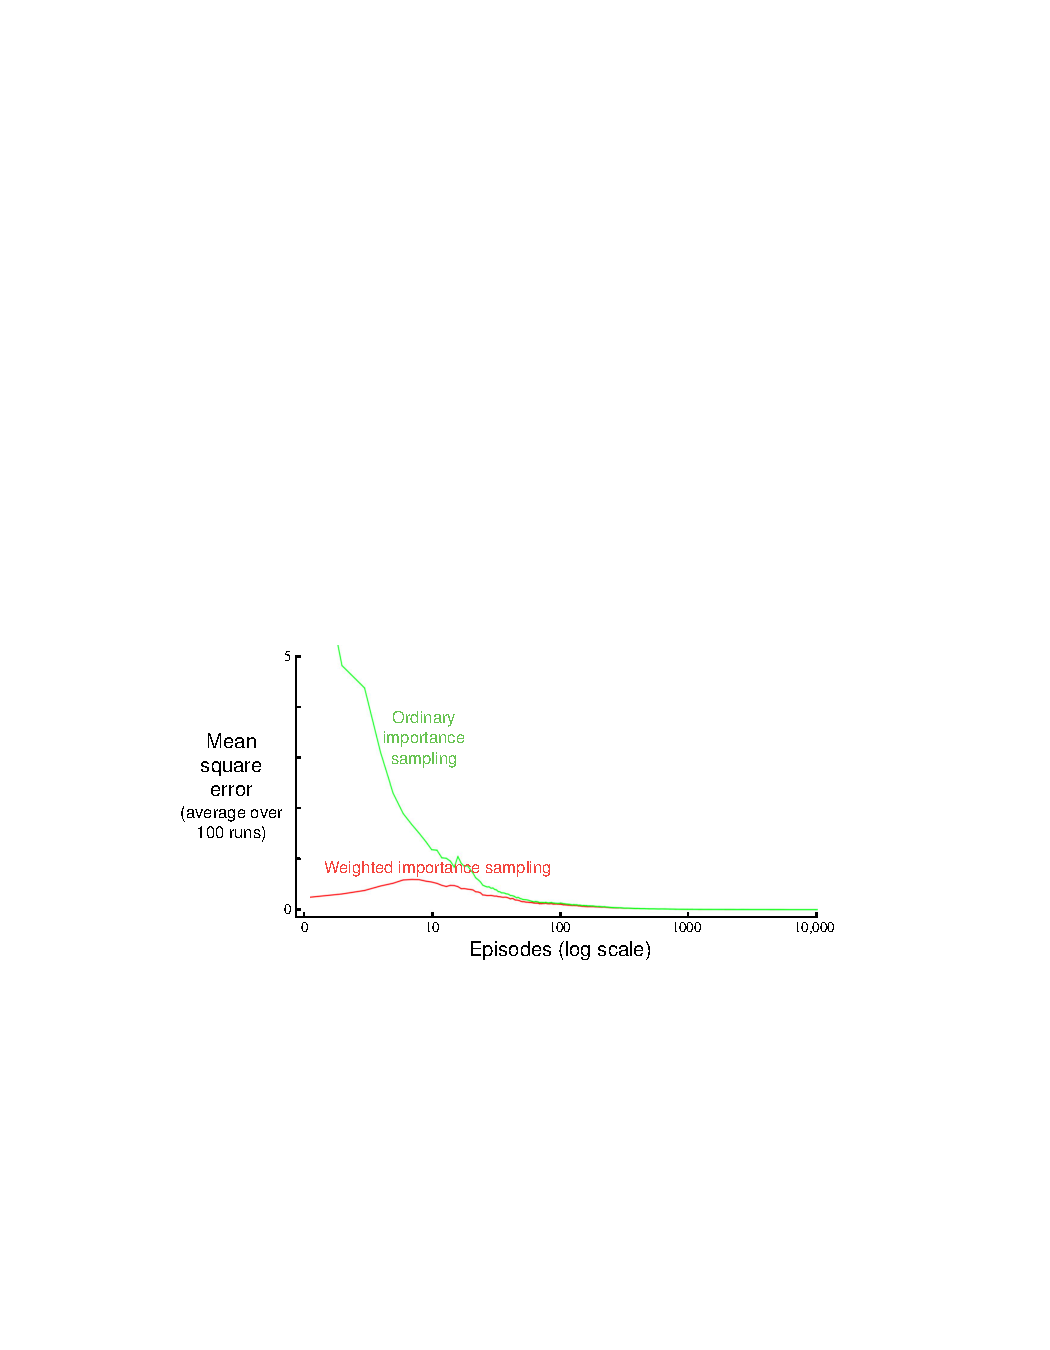
\includegraphics[width=8cm]{fig/lec04/Importance_Sampling_Blackjack.pdf}
	\caption{Off-policy state-value estimation of single state $\{$dealer's sum = 2, player's sum = 13 and player has usable ace$\}$ (source: R. Sutton and G. Barto, Reinforcement learning: an introduction, 2018, \href{https://creativecommons.org/licenses/by-nc-nd/2.0/}{CC BY-NC-ND 2.0})}
	\label{fig:Importance_Sampling_Blackjack}
\end{figure}
}

%%%%%%%%%%%%%%%%%%%%%%%%%%%%%%%%%%%%%%%%%%%%%%%%%%%%%%%%%%%%%
%% Weighted Importance Sampling: Incremental Implementation %%
%%%%%%%%%%%%%%%%%%%%%%%%%%%%%%%%%%%%%%%%%%%%%%%%%%%%%%%%%%%%%
\frame{\frametitle{WIS: Incremental Implementation}
\begin{itemize}
	\item For OIS, \eqref{eq:OIS} can be directly transformed into an incremental implementation following \eqref{eq:inc_impl_MC_pred}.\pause
	\item For WIS an incremental implementation is also highly desirable to save memory and computational resources.\pause
	\item Rewrite WIS \eqref{eq:WIS_MC} for a sequence of returns $g_1, g_2,\ldots$:
	\begin{equation}
		\hat{v}_i(x) = \frac{\sum_{k=1}^{i-1} w_k g_k}{\sum_{k=1}^{i-1} w_k} \quad \mbox{with} \quad w_k=\rho_{k:T(k)} .
	\end{equation}\pause
	\item The WIS recursive/incremental update rule is then:
	\begin{align}
	\hat{v}_{i+1}(x) &= \hat{v}_{i}(x) + \frac{w_i}{c_i}\left(g_i - \hat{v}_{i}(x)\right),\quad i \geq 1 \\
	c_{i+1} &= c_i + w_{i+1} \quad \mbox{with} \quad c_0=0.
	\end{align}
	\item Above, $c_i$ is the cumulative sum of weights over all considered state visits.
\end{itemize}
}

%%%%%%%%%%%%%%%%%%%%%%%%%%%%%%%%%%%%%%%%%%%%%%%%%%%%%%%%%%%%%
%% Algorithmic Implementation: MC-Based Off-Policy Prediction Using WIS %%
%%%%%%%%%%%%%%%%%%%%%%%%%%%%%%%%%%%%%%%%%%%%%%%%%%%%%%%%%%%%%
\frame{\frametitle{MC-Based Off-Policy Prediction Using WIS}
\setlength{\algomargin}{0.5em}
\begin{algorithm}[H]
\footnotesize
\SetKwInput{Input}{input} 
\SetKwInput{Output}{output}
\SetKwInput{Init}{init}
\SetKwInput{Param}{parameter}
\Input{a target policy $\pi$ to be evaluated}
\Init{$\hat{q}(x,u)$ arbitrarily $\forall \, \left\{x\in\mathcal{X}, u\in\mathcal{U}\right\}$\newline 
$c(x,u)\leftarrow 0$ cumulative sum of WIS weights $\forall \, \left\{x\in\mathcal{X}, u\in\mathcal{U}\right\}$}
 \For{$j=1,\ldots,J$ episodes}{
	Choose an arbitrary behavior policy $b$ with coverage of $\pi$\;
	Generate an episode following $b$: $x_{0}, u_{0}, r_{1},\ldots,x_{T_j}, u_{T_j}, r_{T_{j+1}}$ \;
	Set $g \leftarrow 0$\;
	Set $w \leftarrow 1$\;
	\For{$k=T_i-1, T_i-2, T_i-3,\ldots, 0$ time steps while $w \neq 0$}{
				$g \leftarrow \gamma g + r_{k+1}$\;
				$c(x_k,u_k) \leftarrow c(x_k,u_k) + w$\;
				$\hat{q}(x_k,u_k) \leftarrow \hat{q}(x_k,u_k)+\frac{w}{c(x_k,u_k)}\left(g - \hat{q}(x_k,u_k)\right)$\;
				$w \leftarrow w\frac{\pi(u_k|x_{k})}{b(u_k|x_{k})}$\;				
	}
}
\caption{MC-based off-policy prediction using WIS}
\label{algo:MC_off_policy_pred_WIS}
\end{algorithm}
}

%%%%%%%%%%%%%%%%%%%%%%%%%%%%%%%%%%%%%%%%%%%%%%%%%%%%%%%%%%%%%
%% MC-Based Off-Policy Prediction Using WIS: Forest Tree MDP %%
%%%%%%%%%%%%%%%%%%%%%%%%%%%%%%%%%%%%%%%%%%%%%%%%%%%%%%%%%%%%%
\frame{\frametitle{MC-Based Off-Policy Prediction: Forest Tree MDP}
\begin{itemize}
	\item Behavior policy $b$: '\textit{fifty-fifty}'
	\item Target policy $\pi$: optimal policy from \figref{fig:Forest_Markov_Decision_Process_Optimal_Action_Value}
\end{itemize}
\vspace{-0.5cm}
\begin{figure}	
	\hspace*{-1.0cm}
	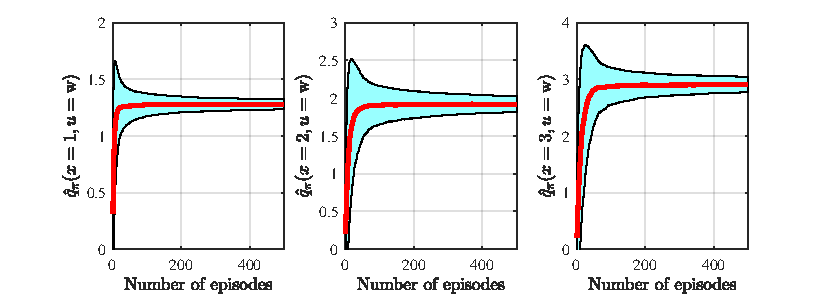
\includegraphics{fig/lec04/Forest_Tree_MC_Off_Policy_Prediction_WIS.pdf}
	\caption{Action-value estimates of forest tree MDP ($\alpha=0.2, \gamma=0.8$) using MC-based off-policy prediction with WIS over the number of episodes. Mean is red and standard deviation is light blue, both calculated based on 2000 independent runs.}
	\label{fig:Forest_Tree_MC_Off_Policy_Prediction_WIS}
\end{figure}
}

%%%%%%%%%%%%%%%%%%%%%%%%%%%%%%%%%%%%%%%%%%%%%%%%%%%%%%%%%%%%%%%%%%
\section{Monte Carlo Off-Policy Control} 
%%%%%%%%%%%%%%%%%%%%%%%%%%%%%%%%%%%%%%%%%%%%%%%%%%%%%%%%%%%%%%%%%%
\begin{frame}
\frametitle{Table of Contents}
\tableofcontents[currentsection]
\end{frame}

%%%%%%%%%%%%%%%%%%%%%%%%%%%%%%%%%%%%%%%%%%%%%%%%%%%%%%%%%%%%%
%% Off-Policy Monte Carlo Control: Introduction %%
%%%%%%%%%%%%%%%%%%%%%%%%%%%%%%%%%%%%%%%%%%%%%%%%%%%%%%%%%%%%%
\frame{\frametitle{Off-Policy Monte Carlo Control: Introduction}
Just put everything together:
\begin{itemize}
	\item MC-based control utilizing GPI (cf. \figref{fig:GPI_MC}),
	\item Off-policy learning based on \algoref{algo:MC_off_policy_pred_WIS}.
\end{itemize}
\vspace{1cm}
Requirement for off-policy MC-based control:
\begin{itemize}
	\item \hl{Coverage}: behavior policy $b$  has nonzero probability of selecting actions that might be taken by the target policy $\pi$.
	\item Consequence: behavior policy $b$ is \hl{soft} (e.g. $\varepsilon$-soft).  
\end{itemize}
}

%%%%%%%%%%%%%%%%%%%%%%%%%%%%%%%%%%%%%%%%%%%%%%%%%%%%%%%%%%%%%
%% Algorithmic Implementation: MC-Based Off-Policy Control Using WIS %%
%%%%%%%%%%%%%%%%%%%%%%%%%%%%%%%%%%%%%%%%%%%%%%%%%%%%%%%%%%%%%
\frame{\frametitle{MC-Based Off-Policy Control Using WIS}
\vspace{-0.175cm}
\setlength{\algomargin}{0.5em}
\begin{algorithm}[H]
\footnotesize
\SetKwInput{Input}{input} 
\SetKwInput{Output}{output}
\SetKwInput{Init}{init}
\SetKwInput{Param}{parameter}
\Init{$\hat{q}(x,u)$ arbitrarily $\forall \, \left\{x\in\mathcal{X}, u\in\mathcal{U}\right\}$\newline 
$c(x,u)\leftarrow 0$ cumulative sum of WIS weights $\forall \, \left\{x\in\mathcal{X}, u\in\mathcal{U}\right\}$\newline
$\pi(x) \leftarrow \argmax_{u} \hat{q}(x,u)$ (with ties broken consistently)}
 \For{$j=1,\ldots,J$ episodes}{
	Choose an arbitrary soft policy $b$\;
	Generate an episode following $b$: $x_{0}, u_{0}, r_{1},\ldots,x_{T_j}, u_{T_j}, r_{T_{j+1}}$ \;
	Set $g \leftarrow 0$\;
	Set $w \leftarrow 1$\;
	\For{$k=T_i-1, T_i-2, T_i-3,\ldots, 0$ time steps}{
				$g \leftarrow \gamma g + r_{k+1}$\;
				$c(x_k,u_k) \leftarrow c(x_k,u_k) + w$\;
				$\hat{q}(x_k,u_k) \leftarrow \hat{q}(x_k,u_k)+\frac{w}{c(x_k,u_k)}\left(g - \hat{q}(x_k,u_k)\right)$\;
				$\pi(x_k) \leftarrow \argmax_{u_k} \hat{q}(x_k,u_k)$ (with ties broken consistently)\;
				\If{$u_k\neq\pi(x_k)$}{
						break/exit inner loop\;
				}
				$w \leftarrow w\frac{1}{b(u_k|x_{k})}$\;
	}
}
\caption{MC-based off-policy control using WIS}
\label{algo:MC_off_policy_control_WIS}
\end{algorithm}
}

%%%%%%%%%%%%%%%%%%%%%%%%%%%%%%%%%%%%%%%%%%%%%%%%%%%%%%%%%%%%%
%% MC-Based Off-Policy Control Using WIS: Forest Tree MDP %%
%%%%%%%%%%%%%%%%%%%%%%%%%%%%%%%%%%%%%%%%%%%%%%%%%%%%%%%%%%%%%
\frame{\frametitle{MC-Based Off-Policy Control: Forest Tree MDP}
\begin{itemize}
	\item Behavior policy $b$: '\textit{fifty-fifty}'
	\item Initial target policy $\pi$: '\textit{fifty-fifty}'
\end{itemize}
\vspace{-0.5cm}
\begin{figure}	
	\hspace*{-1.0cm}
	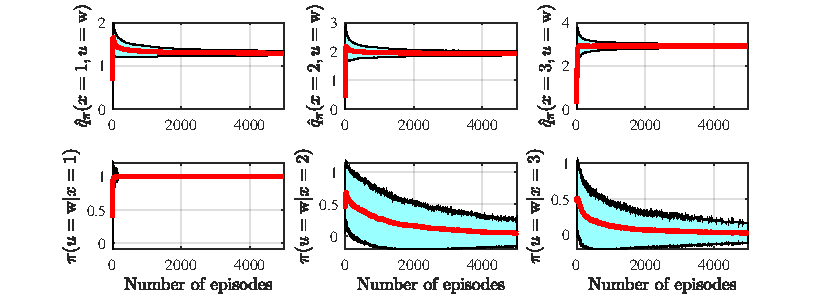
\includegraphics{fig/lec04/Forest_Tree_MC_Off_Policy_Control_WIS.pdf}
	\caption{Action-value estimates and policy trends of forest tree MDP ($\alpha=0.2, \gamma=0.8$) using MC-based off-policy control with WIS over the number of episodes. Mean is red and standard deviation is light blue, both calculated based on 2000 independent runs.}
	\label{fig:Forest_Tree_MC_Off_Policy_Control_WIS}
\end{figure}
}

%%%%%%%%%%%%%%%%%%%%%%%%%%%%%%%%%%%%%%%%%%%%%%%%%%%%%%%%%%%%%
%% Remark on MC-Based Off-Policy Control with WIS %%
%%%%%%%%%%%%%%%%%%%%%%%%%%%%%%%%%%%%%%%%%%%%%%%%%%%%%%%%%%%%%
\frame{\frametitle{Remark on MC-Based Off-Policy Control with WIS}
Potential problems with MC-based off-policy control:
\begin{itemize}
	\item Learns only 'from tails' of episodes if the remaining actions generated by $b$ are greedy with respect to $\pi$. 
	\begin{itemize}
		\item See last and inner-most \textit{if} query in \algoref{algo:MC_off_policy_control_WIS}.
		\item Hence, a lot of samples generated by $b$ remain unused for training $\pi$.
	\end{itemize}\pause
	\item Slows down training.
	\item Adds uncertainty to the training process. 
\end{itemize}
\vspace{0.5cm}\pause
Possible improvements/extensions:
\begin{enumerate}
	\item \hl{Per-decision importance sampling}
	\item \hl{Discounting-aware importance sampling} (if discount factor $\gamma<1$)
\end{enumerate}
\begin{itemize}
	\item Introduce modified value estimators for importance sampling.
	\item Main goal: decrease variance of the learning process.
	\item For details see chapter 5.8 \& 5.9 of R. Sutton and G. Barto, Reinforcement learning: an introduction, 2018 .
\end{itemize}
}

%%%%%%%%%%%%%%%%%%%%%%%%%%%%%%%%%%%%%%%%%%%%%%%%%%%%%%%%%%%%%
%% Summary %%
%%%%%%%%%%%%%%%%%%%%%%%%%%%%%%%%%%%%%%%%%%%%%%%%%%%%%%%%%%%%%
\begin{frame}
\frametitle{Summary: What You've Learned Today}
\begin{itemize}
	\item MC methods allow model-free learning of value functions and optimal policies from experience in the form of sampled episodes.
	\item Using deep back-ups over full episodes, MC is largely based on averaging returns. \pause
	\item MC-based control reuses generalized policy iteration (GPI) i.e. mixing policy evaluation and improvement. \pause
	\item Maintaining sufficient exploration is important:
	\begin{itemize}
		\item Exploring starts: not feasible in all applications but simple.
		\item On-policy $\varepsilon$-greedy learning: trade-off between optimality and exploration cannot be resolved easily.
		\item Off-policy learning: agent learns about a (possibly deterministic) target policy from an exploratory, soft behavior policy.
	\end{itemize}\pause
	\item Importance sampling transforms expectations from the behavior to the target policy.
	\begin{itemize}
		\item This estimation task comes with a bias-variance-dilemma.
		\item Slow learning can result from ineffective experience usage in MC methods.
	\end{itemize}
\end{itemize}
\end{frame}

%%%%%%%%%%%%%%%%%%%%%%%%%%%%%%%%%%%%%%%%%%%%%%%%%%%%%%%%%%%%%
%% Final Slide %%
%%%%%%%%%%%%%%%%%%%%%%%%%%%%%%%%%%%%%%%%%%%%%%%%%%%%%%%%%%%%%
\frame{\frametitle{The End for Today}
\begin{figure}

\includegraphics[width=10cm]{fig/lec04/Dilbert.png}
\end{figure}
\vspace{1cm}
\centering
Thanks for your attention and have a nice week!
}